\documentclass{article}

\usepackage[utf8]{inputenc} % for UTF-8 support
\usepackage[T1]{fontenc} % for font encoding
\usepackage{lipsum} % for sample text
\usepackage[utf8]{inputenc}
\usepackage{float}
\usepackage{graphicx}
\usepackage[backend=biber]{biblatex}
\usepackage[table,xcdraw]{xcolor}
\usepackage[english]{babel}
\usepackage[toc,page]{appendix}
\usepackage[toc,acronym,section]{glossaries} % Acronyms in a nice way
\usepackage[colorinlistoftodos]{todonotes}
\usepackage{caption}
\usepackage{subcaption}
\usepackage{listings}
\usepackage{csquotes}
\usepackage{titlesec}

\setlength\parindent{0pt}

\titleformat*{\section}{\LARGE\bfseries}
\titleformat*{\subsection}{\Large\bfseries}
\titleformat*{\subsubsection}{\large\bfseries}
\titleformat*{\paragraph}{\large\bfseries}
\titleformat*{\subparagraph}{\large\bfseries}

\usepackage[a4paper,
            bindingoffset=0.2in,
            left=1in,
            right=1in,
            top=1in,
            bottom=1in,
            footskip=.25in]{geometry}

\begin{document}

%----------------------------------------------------------------------------------------
%	FRONTPAGE
%----------------------------------------------------------------------------------------

\begin{titlepage}

\newcommand{\HRule}{\rule{\linewidth}{0.5mm}} 
\center

%----------------------------------------------------------------------------------------
%	HEADING SECTIONS
%----------------------------------------------------------------------------------------


\includegraphics[scale=0.15]{report/images/ITU.jpg}\\[3cm]

\textsc{\LARGE DevOps, Software Evolution and Software Maintenance (Spring 2023)}\\[0.5cm] % Major heading such as course name
Course Code: KSDSESM1KU\\[1cm]

%----------------------------------------------------------------------------------------
%	TITLE SECTION
%----------------------------------------------------------------------------------------

\HRule \\[0.8cm]
{ \huge \bfseries Exam project: MiniTwit }\\[0.4cm] % Title of your document
\HRule \\[1.5cm]

%----------------------------------------------------------------------------------------
%	AUTHOR SECTION
%----------------------------------------------------------------------------------------

\begin{minipage}{0.6\textwidth}
    \center
    \emph{Students:}\\
    Gustav Vilain Brygger - gubr@itu.dk \\
    Niklas Brynfeldt - nbry@itu.dk \\
    Bjarke Dalhoff Christensen - bjch@itu.dk \\
    Oliver Simon Jarvis - ojar@itu.dk \\
    Amanda Rasille Røn Volf - amav@itu.dk \\

\end{minipage}\\[2cm]

%----------------------------------------------------------------------------------------
%	DATE SECTION
%----------------------------------------------------------------------------------------
{\large \today}\\[2cm]

\vfill % Fill the rest of the page with whitespace

\end{titlepage}

\pagenumbering{gobble} % Remove page numbering
\newpage

\tableofcontents
\newpage

\pagenumbering{arabic}

%----------------------------------------------------------------------------------------
%	REPORT
%----------------------------------------------------------------------------------------

\section{Introduction}
This report will contain a systematic description and illustration of the Go application 
'MiniTwit'. The application was developed as part of the course 
DevOps, Software Evolution and Software Maintenance (Spring 2023). \\

The functionality of the application was
given in a similar application written in Python and Flask provided as part of the course material. This
application was outdated and the structure was suboptimal. Thus, we rewrote this application to a more 
maintainable system. Our developed application was able to handle registering users, login/logout, 
posting messages, and follow/unfollow functionality. The application consisted of a user interface, 
as seen in figure \ref{fig:minitwit_app}, as well as endpoints used by a simulator throughout the course to 
mimic real users' interactions with our application.

\begin{figure}[H]
    \centering
    \captionsetup{justification=centering,margin=1cm}
    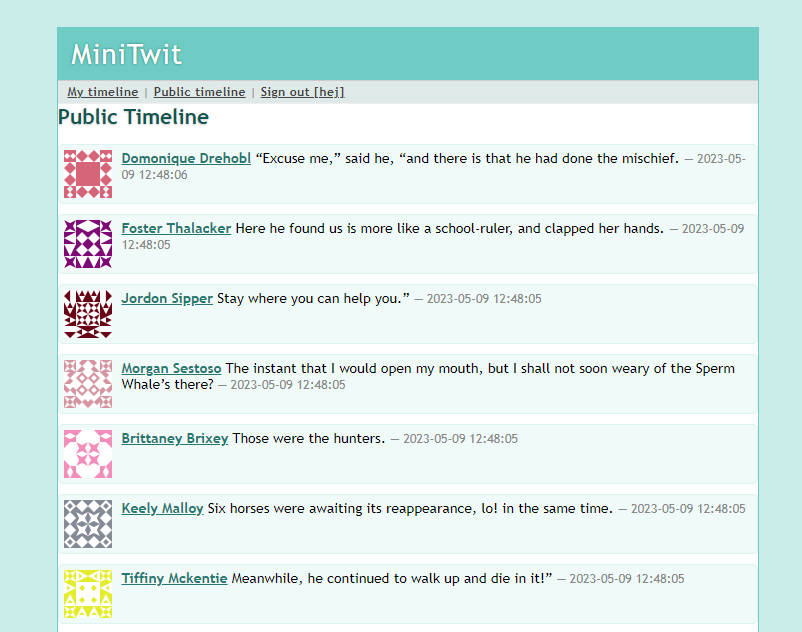
\includegraphics[width=0.8\linewidth]{report/images/minitwit.png}
    \caption{MiniTwit Application Frontend}
    \label{fig:minitwit_app}
\end{figure}

If any errors were detected by the simulator, for instance, if the wrong response was received or if the system
responded too slowly, these would be logged to allow us to handle them appropriately.\\

The rest of this report will explain the application from different perspectives and finally reflect upon
what we learned throughout the project.

\section{Links}
Below can be find the links for our attributes:
\begin{itemize}
    \item Repository URL: \href{https://github.com/organizationGB/DevOps}
    \item Monitoring URL: \href{http://206.189.48.173:3000/d/E4amSsB4k/minitwit-monitoring?orgId=1&from=1681196813508&to=1681207613508}
    \item Security Assessment report URL: \href{https://github.com/organizationGB/DevOps/blob/main/securityassesment.md}
    \item Logging URL: \href{http://206.189.48.173:5601/}
    \item SLA URL: \href{https://github.com/organizationGB/DevOps/blob/main/SLA.md}
    \item Application URL: \href{http://206.189.48.173:8080/}
\end{itemize}
\section{System's Perspective}

\subsection{Design and Architecture of MiniTwit}
The MiniTwit application architecture has been designed by following some important software design guidelines 
such as low coupling, high cohesion, and the Single Responsibility Principle(SRP). 
These concepts are closely related and basing the development on those helped us create software that is easier to work with. 

The SRP states that each part of a software system should be responsible for one thing and therefore only have one reason to change(KILDE). 
Cohesion is closely related to the SRP and it is a measure of the degree to which related functionality is grouped together in a single coherent unit(KILDE). 
In general, the goal is to have modules with high cohesion as this ensures that the code in a given module is focused on a single aspect of the application's functionality. 
This is important as having too much functionality in a single module is likely to result in code that is hard to both understand and change. 

Finally, coupling refers to the degree of interdependence between the modules within a system and it measures how well-defined the boundaries between different modules are. 
Coupling can be classified as either low or high and low coupling implies that modules' knowledge of other modules' internal implementation details have been minimized(KILDE).
Together the SRP, low coupling, and high cohesion are key enablers when it comes to reducing complexity and thereby ensuring a strong foundation for designing extendable software. \\

To achieve low coupling and high cohesion the MiniTwit application has been split into three layers namely persistence, web, and application as seen in figure \ref{fig:minitwit}. 
As prescribed by the SRP each layer is responsible for one thing and we have minimized the dependencies between the layers thus making it easier to extend MiniTwit with new features. 
It also reduces cognitive load as it makes it easier to navigate the system because code related to the same functionality is grouped together. 


% Fix system architecture image.
\begin{figure}[H]
    \centering
    \captionsetup{justification=centering,margin=1cm}
    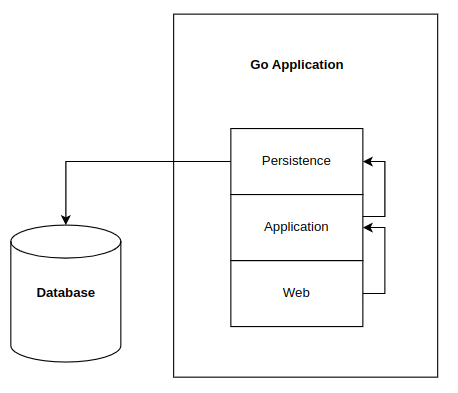
\includegraphics[width=0.8\linewidth]{./images/system_architecture.png}
    \caption{MiniTwit Architecture}
    \label{fig:minitwit}
\end{figure}



\subsubsection{Application, Persistence, and Web}
In the application layer, all code related to core business logic is found. This includes the models that MiniTwit is built upon such as User and Message. 
Business logic has been separated from other parts of the application as doing so allows developers to understand and 
modify business logic without impacting other components of the application. Secondly, separating business logic promotes reusability, 
as the code can easily be shared across different parts of the application.     \\

In the persistence layer, the database setup is configured. We use an Object Relational Mapper(ORM) called GORM to interact 
with the database as it abstracts some of the complexity that comes with a relational database(Link to ORM section). 
Migrations and data seed are also handled in the persistence layer the latter only when the database contains no data. 
This is useful for local development and in test environments as the application can be tested without having to create users first. \\

The web layer is implemented using a lightweight Go web framework called Gin. 
Gin was chosen because it offers a minimalistic and fast approach to building web applications as it provides 
essential features like routing, middleware support, JSON handling, and request/response binding(KILDE). 
All features that would have taken a long time to implement from scratch. Gin route requests to controllers 
which coordinate the request/response cycle which includes ensuring the validity of a given request. 
Some requests include new data such as tweets and this data is used to update the database state after 
which HTML containing the updated state is generated and returned to the client. 


\subsection{Dependencies of MiniTwit system}

For the MiniTwit application to run we are depending on first and foremost Digital Ocean whos servers the application is 
hosted on. The servers are running 9 docker containers responsible for: 
\begin{itemize}
    \item The Database running on a postgres:14.1-alpine image - Responsible for holding all the users data.
    \item The Server itself running on a golang:bullseye image.
    \item A redis server for storing sessions and the integer 'latest'.
    \item Elastic Search - Indexing logs such that we can search and analyse them
    \item Filebeat for collecting and forwarding the logging to Elastic search
    \item Kibana for visualizing the results from Elastic search
    \item Prometheus for monitoring the application in terms of CPU usage and request time
    \item Grafana for visualizing the monitoring
    \item Nginx for load balancing the incoming traffic to the different services
\end{itemize}

From within each of these containers we depend on large number of libraries of which the major ones we consider to be:
\begin{itemize}
    \item Gorm used for object-relational mapping allowing us to perform CRUD operations io GO.
    \item Gin handling all of the routing of the HTTP methods.
    \item x/crypto/bcrypt library for hashing the user password.
\end{itemize}

For initializing the containers we used docker-compose and docker swarm. Hence we also depend on docker, docker-compose
and terraform which was used to init all the servers
\begin{itemize}
    \item connect to docker swarm nodes via token
    \item manage ssh keys on nodes 
    \item mange config an secret on notes
\end{itemize}

In a more board sense the application also depend on Go, Ubuntu, python and SSH protocol to work. At last we 
also depend on pre-build git workflows such as \textit{docker/build-push-action@v2} or \textit{rymndhng/release-on-push-action@master}.

%OBS MSc students: Remember to log and provide good arguments for the choice of programming language and framework
\subsubsection{Arguments for programming language and framework}
We initially set out to use FastAPI in Python, but eventually settled on GO for multiple reasons. From a personal 
development perspective, learning a new language is rarely a poor choice. Go is well-known for being relatively 
fast to learn, whilst maintaining speed. From a more technical perspective Go has advantages over many languages. 
It's fast, it has concurrency built-in, and it has a strong standard library support, with most important features, 
even templating, being available as a standard package.\\

Gin is not the fastest Go framework, but it has several advantages. It is well-maintained, has over twice the 
amount of github stars than the next most popular framework, and is one of the faster go web frameworks.\\

Whilst implementing the application in fastAPI might have been faster and easier, due to both prior python 
knowledge, and general simplicity, the advantages of using go with the GIN framework can't be overstated. 

%OBS MSc students: Remember to log and provide good arguments for the choice of virtualization techniques and deployment targets
\subsubsection{Arguments for virtualization techniques and deployment targets}
Docker was chosen because it's the industry standard. Other container strategies are good, but given knowledge 
of future need for orchestration (in either docker swarm or kubernetes) Docker was an obvious choice.\\

We used Digital Ocean mainly for budgetary reasons and for ease of deployment. Using the Github Student 
Starter pack, \$200 in free credits were made available to us. This was enough to ensure that the application 
was able to run for the duration of the course. In fact it allowed us to test out the different deployment strategies
from monoroid and containerized application being spin up with only docker-compose to more advanced strategies such as
running on multiple servers with services running to mimimize downtime.\\

Using multiple accounts furthermore allowed us to create a parallel Digital ocean was employed for budgetary reasons, and also because the guides were made for it.
It's also more accessible than other more complicated providers such as AWS. 

\subsubsection{Arguments for ORM and DBMS}
%OBS MSc students: Remember to log and provide good arguments for the choice of ORM framework and chosen DBMS.
In regards to choosing ORM(Object-relational mapping) and DBMS(Database Management Systems) we settled on 
using \textit{PostgresSQL} as our DBMS and \textit{Gorm} for ORM. In terms of choosing DBMS we considered 
\textit{SQLite} and \textit{digital ocean manged db}:
\begin{itemize}
    \item Potential arguments over SQLite 
    \begin{itemize}
        \item Scalability
        \item Concurrency
        \item No user management
        \item Network access        
    \end{itemize}
    \item Potential arguments over e.g. digital ocean manged db
    \begin{itemize}
        \item Cost
    \end{itemize}
\end{itemize}

For ORM we considered \textit{XORM} and \textit{beego} but due to our limited experience with GO we choose Gorm 
since it widely used, well documented and has better superior features like sanitizing input \footnote{\url{https://blog.logrocket.com/comparing-orm-packages-go/ & https://sumit-agarwal.medium.com/gorm-vs-xorm-part-1-d156ba9de404}}.


\subsubsection{Arguments for Terraform}
% Argue for Terraform choice??
- Infrastructure as code is important for maintainability reasons. Therefore Terraform was an obvious choice.
Terraform is for remote cloud providers. Vagrant is for local development. 

\subsection{Important Interactions of Subsystems}
In the image below the interactions between our subsystems can be seen:

\begin{figure}[H]
    \centering
    \captionsetup{justification=centering,margin=1cm}
    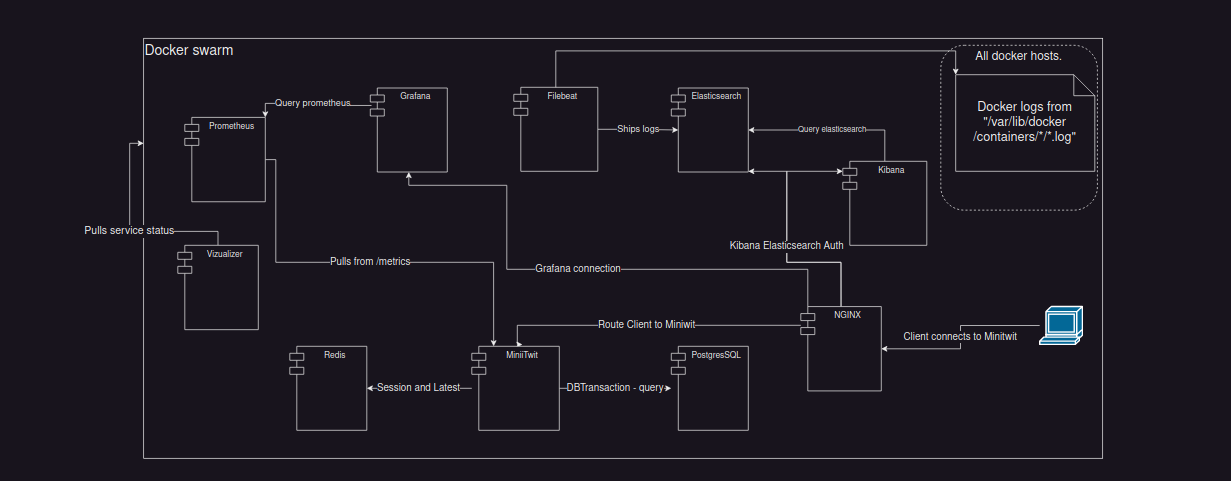
\includegraphics[width=0.8\linewidth]{report/images/InteractionsOfSystems.png}
    \caption{Subsystem interactions}
    \label{fig:minitwit}
\end{figure}

\subsection{Current state of the system}
In the current state of the system our stack consists of: 
\begin{itemize}
    \item Application running on Digital Ocean
    \item Run tests in CI/CD pipeline within an isolated environment
    \item Monitoring the application with Prometheus and Grafana
    \item Code quality checks using Golangci-lint in the CI/CD pipeline checking for typecheck, gosimple, unused etc.
    \item Logging using elastic search and Kibana
\end{itemize}
We did not manage to get Docker swarm and Redis up and running. Docker swarm were missing to be setup 
in our CI/CD chain and Redis seemed to be running locally but a bug on prod seemed to ruin Redis.

\subsection{Project License}

\section{Process' Perspective}

\subsection{Developer interactions}
Throughout the development of the project during the course, the team has interacted primarily through Discord when remote communication was used. 
Further, the team met physically at ITU on Tuesdays where we communicated with each other during the entire day. 

\subsection{Team organization}
We organized ourselves as a cross-functional team. Sometimes we worked on tasks individually but for the majority of the project we worked together, 
typically in pairs. Every opinion and input from each team member was acknowledged equally. 

\subsection{CI/CD chains}
Our CI/CD chain consists of the following workflows used with GitHub Actions:
\begin{itemize}
    \item Continuous-deployment - Deploys the code of the main branch to production using Docker, ssh onto the server where we run our deployment script.
    \item Dev - Functions as the Continuous-deployment workflow but deploys to a test server.
    \item Test - Runs the test docker-compose file which creates a closed environment with the code on the current branch and runs the test.
    \item Main Release - This uses an extern workflow namely \textit{rymndhng/release-on-push-action@master} for creating a release every time a push to main is made.
    \item Lint - Uses the external workflow 'golangci/golangci-lint-action@v3' which checks the code with multiple linters.
\end{itemize}

Every time a pull request was made to a branch, the 'Lint' and 'Test' workflows were run. The workflows that handled deployment were triggered manually.
Further, we have set up CodeClimate and SonarCloud to help us maintain an appropriate standard of our code base such that we don't introduce new issues
with new features. The SonarCloud check is made every time a pull request is made to our main branch (see section \ref{branching} for a description of the 
branching structure).

\subsection{Organization of Repository}
The project only consists of a single repository containing the application. We chose this because it is a small application and thus splitting it into multiple
repositories would have complicated the development process unnecessarily. This single repository contains several folders, 
each containing different files:

\renewcommand{\arraystretch}{3}
\begin{table}[H]
    \centering
    \resizebox{\textwidth}{!}{%
    \begin{tabular}{|l|l|}
    \hline
    \Large\textbf{.github/workflows} & \Large Contains all our workflow files used with GitHub Actions.                                                                                                          \\ \hline
    \Large\textbf{api\_test}         & \Large Includes files to run the simulator and a test of the API. Primarily used during the development of the endpoints.                                                     \\ \hline
    \Large\textbf{remote\_files}     & \Large Has all files that are used when deploying to the server. This includes various logging and monitoring files, \\ & \Large our deploy script, and the docker-compose file.      \\ \hline
    \Large\textbf{report}            & \Large This folder is where our report files are saved.                                                                                                                   \\ \hline
    \Large\textbf{src}               & \Large Contains all our application code which is further divided into subfolders, thereby separating the logic \\ & \Large of the system.                                            \\ \hline
    \Large\textbf{tests}             & \Large Our test files are located in this folder. It contains a Docker file, a docker-compose file, and a test file to \\ &  \Large run our tests without external impact. \\ \hline
    \end{tabular}%
    }
    \caption{Repository folders}
    \label{tab:repo_folders}
    \end{table}

\subsection{Branching strategy} \label{branching}
We used two static branches as part of our branching strategy throughout the development of the project. 
The main branch was used as our primary branch on which only functioning and tested code was meant to be pushed. It was
also the code on this branch we deployed on our main server. The other branch was the dev branch. This was used for 
development and testing. Additional branches were created when new functionality should be implemented, or bugs had to be
fixed. All these temporary branches were derived from the main branch. Our general branching strategy and an example where
we have used this in Github can be seen in figure \ref{fig:gen_branch} and \ref{fig:ex_branch}, respectively:

\begin{figure}[H]
    \centering
    \captionsetup{justification=centering,margin=1cm}
    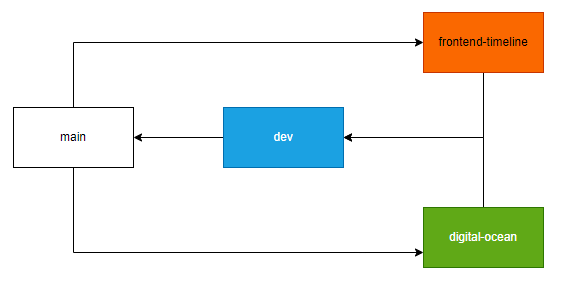
\includegraphics[width=0.7\linewidth]{report/images/branching.png}
    \caption{General branching strategy}
    \label{fig:gen_branch}
\end{figure}

\begin{figure}[H]
    \centering
    \captionsetup{justification=centering,margin=1cm}
    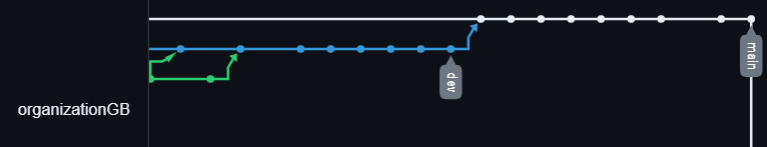
\includegraphics[width=0.7\linewidth]{report/images/git_branching.png}
    \caption{Example use of branching strategy}
    \label{fig:ex_branch}
\end{figure}

It can be seen that the temporary branches are derived from the main branch, and when the functionality is implemented, 
it is merged into the dev branch to be tested before the code is put into production. 

\subsection{Development process and tools}
Usually, when meeting on Tuesdays we discussed what needed to be done if we weren't already working on a task. We tried to start using a Kanban board but due to us not establishing 
clear guidelines on how to use the tool, we didn't manage to successfully implement it. In our development process, we utilized pair programming a lot. This also lead to a very iterative development 
process in the sense that we pushed small changes often to switch programmer. Further, the team agreed that when larger new implementations were to be introduced
to the main or dev branch, a pull request should be made to allow another team member to review the code and ensure that the workflows would catch any newly
introduced issues. 

\subsection{Monitoring}
The deployed MiniTwit application was monitored using Grafana, which is a dashboard web application for visualization of data. 
We used Grafana to monitor the simulator's interaction with our application and other parameters of the system. On our dashboard, 
we included a visualization of the CPU load percentage as well as an overview of the duration of requests to the different endpoints  
we got. Here it was possible to select a single endpoint and see the metrics for that type of request. This allowed us to analyze why 
there were higher CPU loads sometimes as this might be due to a resource-intensive request. Additionally, we monitored the total number of
responses to allow us to monitor the availability of the application. \\

To collect this data for visualization, we used Prometheus as it is an open-source monitoring system that can be used to collect 
and store various metrics data from the web server. Prometheus pulls the metric data from the MiniTwit application from an exposed metrics endpoint
and stores it so it can be queried by Grafana and shown in the dashboard.  

\subsection{Logging}
Not finished yet

\subsection{Security assessment}
From our security assessment, we learned that the risks with the highest likelihood were that an attacker could gain unauthorized access to our codebase
and our weak authentication and authorization mechanisms. The first risk was likely to occur as it was possible to find passwords and usernames for the database 
in our public codebase. We made sure that these are not stored directly in the source code by importing them from GitHub secrets instead. The second identified 
risk could be improved by changing the default usernames and passwords used to something that follows security standards.  

\subsection{Scaling and load balancing}
%Docker swarms and 2x nginx as load balancers. 
Not finished yet.

\subsection{AI-assistants}
The team has used AI-assistants to aid in the development and deployment of the MiniTwit application. We used OpenAI's ChatGPT, which is an AI language model, 
and Phind, which is an AI search engine. They were used to provide general information regarding the technologies we used as well as how to approach development tasks,
such as describing the different components used in a docker-compose file or implementing a Go application using the Gin framework. \\
  
Using these assistants aided us because they provided a quick overview of the possibilities with short explanations. They gave us a way to quickly get started with
implementation in a language we did not know as it suggested code in which we were quickly able to learn the syntax of Go and how to structure our application. However, 
using them also hindered us as we often had to double-check whether the information provided was accurate and so ended up using more time than if we obtained the information 
without them. 
\section{Lessons Learned Perspective}

\subsection{Evolution and Refactoring}

\subsection{Operation}

\subsection{Maintenance}

\end{document}